%%
% Copyright (c) 2017 - 2023, Pascal Wagler;
% Copyright (c) 2014 - 2023, John MacFarlane
%
% All rights reserved.
%
% Redistribution and use in source and binary forms, with or without
% modification, are permitted provided that the following conditions
% are met:
%
% - Redistributions of source code must retain the above copyright
% notice, this list of conditions and the following disclaimer.
%
% - Redistributions in binary form must reproduce the above copyright
% notice, this list of conditions and the following disclaimer in the
% documentation and/or other materials provided with the distribution.
%
% - Neither the name of John MacFarlane nor the names of other
% contributors may be used to endorse or promote products derived
% from this software without specific prior written permission.
%
% THIS SOFTWARE IS PROVIDED BY THE COPYRIGHT HOLDERS AND CONTRIBUTORS
% "AS IS" AND ANY EXPRESS OR IMPLIED WARRANTIES, INCLUDING, BUT NOT
% LIMITED TO, THE IMPLIED WARRANTIES OF MERCHANTABILITY AND FITNESS
% FOR A PARTICULAR PURPOSE ARE DISCLAIMED. IN NO EVENT SHALL THE
% COPYRIGHT OWNER OR CONTRIBUTORS BE LIABLE FOR ANY DIRECT, INDIRECT,
% INCIDENTAL, SPECIAL, EXEMPLARY, OR CONSEQUENTIAL DAMAGES (INCLUDING,
% BUT NOT LIMITED TO, PROCUREMENT OF SUBSTITUTE GOODS OR SERVICES;
% LOSS OF USE, DATA, OR PROFITS; OR BUSINESS INTERRUPTION) HOWEVER
% CAUSED AND ON ANY THEORY OF LIABILITY, WHETHER IN CONTRACT, STRICT
% LIABILITY, OR TORT (INCLUDING NEGLIGENCE OR OTHERWISE) ARISING IN
% ANY WAY OUT OF THE USE OF THIS SOFTWARE, EVEN IF ADVISED OF THE
% POSSIBILITY OF SUCH DAMAGE.
%%

%%
% This is the Eisvogel pandoc LaTeX template.
%
% For usage information and examples visit the official GitHub page:
% https://github.com/Wandmalfarbe/pandoc-latex-template
%%

% Options for packages loaded elsewhere
\PassOptionsToPackage{unicode}{hyperref}
\PassOptionsToPackage{hyphens}{url}
\PassOptionsToPackage{dvipsnames,svgnames,x11names,table}{xcolor}
%
\documentclass[
  paper=a4,
  ,captions=tableheading
]{scrartcl}
\usepackage{amsmath,amssymb}
% Use setspace anyway because we change the default line spacing.
% The spacing is changed early to affect the titlepage and the TOC.
\usepackage{setspace}
\setstretch{1.2}
\usepackage{iftex}
\ifPDFTeX
  \usepackage[T1]{fontenc}
  \usepackage[utf8]{inputenc}
  \usepackage{textcomp} % provide euro and other symbols
\else % if luatex or xetex
  \usepackage{unicode-math} % this also loads fontspec
  \defaultfontfeatures{Scale=MatchLowercase}
  \defaultfontfeatures[\rmfamily]{Ligatures=TeX,Scale=1}
\fi
\usepackage{lmodern}
\ifPDFTeX\else
  % xetex/luatex font selection
\fi
% Use upquote if available, for straight quotes in verbatim environments
\IfFileExists{upquote.sty}{\usepackage{upquote}}{}
\IfFileExists{microtype.sty}{% use microtype if available
  \usepackage[]{microtype}
  \UseMicrotypeSet[protrusion]{basicmath} % disable protrusion for tt fonts
}{}
\makeatletter
\@ifundefined{KOMAClassName}{% if non-KOMA class
  \IfFileExists{parskip.sty}{%
    \usepackage{parskip}
  }{% else
    \setlength{\parindent}{0pt}
    \setlength{\parskip}{6pt plus 2pt minus 1pt}}
}{% if KOMA class
  \KOMAoptions{parskip=half}}
\makeatother
\usepackage{xcolor}
\definecolor{default-linkcolor}{HTML}{A50000}
\definecolor{default-filecolor}{HTML}{A50000}
\definecolor{default-citecolor}{HTML}{4077C0}
\definecolor{default-urlcolor}{HTML}{4077C0}
\usepackage[margin=2.5cm,includehead=true,includefoot=true,centering,]{geometry}
\usepackage{color}
\usepackage{fancyvrb}
\newcommand{\VerbBar}{|}
\newcommand{\VERB}{\Verb[commandchars=\\\{\}]}
\DefineVerbatimEnvironment{Highlighting}{Verbatim}{commandchars=\\\{\}}
% Add ',fontsize=\small' for more characters per line
\newenvironment{Shaded}{}{}
\newcommand{\AlertTok}[1]{\textcolor[rgb]{1.00,0.00,0.00}{\textbf{#1}}}
\newcommand{\AnnotationTok}[1]{\textcolor[rgb]{0.38,0.63,0.69}{\textbf{\textit{#1}}}}
\newcommand{\AttributeTok}[1]{\textcolor[rgb]{0.49,0.56,0.16}{#1}}
\newcommand{\BaseNTok}[1]{\textcolor[rgb]{0.25,0.63,0.44}{#1}}
\newcommand{\BuiltInTok}[1]{\textcolor[rgb]{0.00,0.50,0.00}{#1}}
\newcommand{\CharTok}[1]{\textcolor[rgb]{0.25,0.44,0.63}{#1}}
\newcommand{\CommentTok}[1]{\textcolor[rgb]{0.38,0.63,0.69}{\textit{#1}}}
\newcommand{\CommentVarTok}[1]{\textcolor[rgb]{0.38,0.63,0.69}{\textbf{\textit{#1}}}}
\newcommand{\ConstantTok}[1]{\textcolor[rgb]{0.53,0.00,0.00}{#1}}
\newcommand{\ControlFlowTok}[1]{\textcolor[rgb]{0.00,0.44,0.13}{\textbf{#1}}}
\newcommand{\DataTypeTok}[1]{\textcolor[rgb]{0.56,0.13,0.00}{#1}}
\newcommand{\DecValTok}[1]{\textcolor[rgb]{0.25,0.63,0.44}{#1}}
\newcommand{\DocumentationTok}[1]{\textcolor[rgb]{0.73,0.13,0.13}{\textit{#1}}}
\newcommand{\ErrorTok}[1]{\textcolor[rgb]{1.00,0.00,0.00}{\textbf{#1}}}
\newcommand{\ExtensionTok}[1]{#1}
\newcommand{\FloatTok}[1]{\textcolor[rgb]{0.25,0.63,0.44}{#1}}
\newcommand{\FunctionTok}[1]{\textcolor[rgb]{0.02,0.16,0.49}{#1}}
\newcommand{\ImportTok}[1]{\textcolor[rgb]{0.00,0.50,0.00}{\textbf{#1}}}
\newcommand{\InformationTok}[1]{\textcolor[rgb]{0.38,0.63,0.69}{\textbf{\textit{#1}}}}
\newcommand{\KeywordTok}[1]{\textcolor[rgb]{0.00,0.44,0.13}{\textbf{#1}}}
\newcommand{\NormalTok}[1]{#1}
\newcommand{\OperatorTok}[1]{\textcolor[rgb]{0.40,0.40,0.40}{#1}}
\newcommand{\OtherTok}[1]{\textcolor[rgb]{0.00,0.44,0.13}{#1}}
\newcommand{\PreprocessorTok}[1]{\textcolor[rgb]{0.74,0.48,0.00}{#1}}
\newcommand{\RegionMarkerTok}[1]{#1}
\newcommand{\SpecialCharTok}[1]{\textcolor[rgb]{0.25,0.44,0.63}{#1}}
\newcommand{\SpecialStringTok}[1]{\textcolor[rgb]{0.73,0.40,0.53}{#1}}
\newcommand{\StringTok}[1]{\textcolor[rgb]{0.25,0.44,0.63}{#1}}
\newcommand{\VariableTok}[1]{\textcolor[rgb]{0.10,0.09,0.49}{#1}}
\newcommand{\VerbatimStringTok}[1]{\textcolor[rgb]{0.25,0.44,0.63}{#1}}
\newcommand{\WarningTok}[1]{\textcolor[rgb]{0.38,0.63,0.69}{\textbf{\textit{#1}}}}

% Workaround/bugfix from jannick0.
% See https://github.com/jgm/pandoc/issues/4302#issuecomment-360669013)
% or https://github.com/Wandmalfarbe/pandoc-latex-template/issues/2
%
% Redefine the verbatim environment 'Highlighting' to break long lines (with
% the help of fvextra). Redefinition is necessary because it is unlikely that
% pandoc includes fvextra in the default template.
\usepackage{fvextra}
\DefineVerbatimEnvironment{Highlighting}{Verbatim}{breaklines,fontsize=\small,commandchars=\\\{\}}

% add backlinks to footnote references, cf. https://tex.stackexchange.com/questions/302266/make-footnote-clickable-both-ways
\usepackage{footnotebackref}
\usepackage{graphicx}
\makeatletter
\def\maxwidth{\ifdim\Gin@nat@width>\linewidth\linewidth\else\Gin@nat@width\fi}
\def\maxheight{\ifdim\Gin@nat@height>\textheight\textheight\else\Gin@nat@height\fi}
\makeatother
% Scale images if necessary, so that they will not overflow the page
% margins by default, and it is still possible to overwrite the defaults
% using explicit options in \includegraphics[width, height, ...]{}
\setkeys{Gin}{width=\maxwidth,height=\maxheight,keepaspectratio}
% Set default figure placement to htbp
\makeatletter
\def\fps@figure{htbp}
\makeatother
\setlength{\emergencystretch}{3em} % prevent overfull lines
\providecommand{\tightlist}{%
  \setlength{\itemsep}{0pt}\setlength{\parskip}{0pt}}
\setcounter{secnumdepth}{-\maxdimen} % remove section numbering
\ifLuaTeX
  \usepackage{selnolig}  % disable illegal ligatures
\fi
\IfFileExists{bookmark.sty}{\usepackage{bookmark}}{\usepackage{hyperref}}
\IfFileExists{xurl.sty}{\usepackage{xurl}}{} % add URL line breaks if available
\urlstyle{same}
\hypersetup{
  hidelinks,
  breaklinks=true,
  pdfcreator={LaTeX via pandoc with the Eisvogel template}}
\author{}
\date{}



%%
%% added
%%


%
% for the background color of the title page
%

%
% break urls
%
\PassOptionsToPackage{hyphens}{url}

%
% When using babel or polyglossia with biblatex, loading csquotes is recommended
% to ensure that quoted texts are typeset according to the rules of your main language.
%
\usepackage{csquotes}

%
% captions
%
\definecolor{caption-color}{HTML}{777777}
\usepackage[font={stretch=1.2}, textfont={color=caption-color}, position=top, skip=4mm, labelfont=bf, singlelinecheck=false, justification=raggedright]{caption}
\setcapindent{0em}

%
% blockquote
%
\definecolor{blockquote-border}{RGB}{221,221,221}
\definecolor{blockquote-text}{RGB}{119,119,119}
\usepackage{mdframed}
\newmdenv[rightline=false,bottomline=false,topline=false,linewidth=3pt,linecolor=blockquote-border,skipabove=\parskip]{customblockquote}
\renewenvironment{quote}{\begin{customblockquote}\list{}{\rightmargin=0em\leftmargin=0em}%
\item\relax\color{blockquote-text}\ignorespaces}{\unskip\unskip\endlist\end{customblockquote}}

%
% Source Sans Pro as the de­fault font fam­ily
% Source Code Pro for monospace text
%
% 'default' option sets the default
% font family to Source Sans Pro, not \sfdefault.
%
\ifnum 0\ifxetex 1\fi\ifluatex 1\fi=0 % if pdftex
    \usepackage[default]{sourcesanspro}
  \usepackage{sourcecodepro}
  \else % if not pdftex
    \usepackage[default]{sourcesanspro}
  \usepackage{sourcecodepro}

  % XeLaTeX specific adjustments for straight quotes: https://tex.stackexchange.com/a/354887
  % This issue is already fixed (see https://github.com/silkeh/latex-sourcecodepro/pull/5) but the
  % fix is still unreleased.
  % TODO: Remove this workaround when the new version of sourcecodepro is released on CTAN.
  \ifxetex
    \makeatletter
    \defaultfontfeatures[\ttfamily]
      { Numbers   = \sourcecodepro@figurestyle,
        Scale     = \SourceCodePro@scale,
        Extension = .otf }
    \setmonofont
      [ UprightFont    = *-\sourcecodepro@regstyle,
        ItalicFont     = *-\sourcecodepro@regstyle It,
        BoldFont       = *-\sourcecodepro@boldstyle,
        BoldItalicFont = *-\sourcecodepro@boldstyle It ]
      {SourceCodePro}
    \makeatother
  \fi
  \fi

%
% heading color
%
\definecolor{heading-color}{RGB}{40,40,40}
\addtokomafont{section}{\color{heading-color}}
% When using the classes report, scrreprt, book,
% scrbook or memoir, uncomment the following line.
%\addtokomafont{chapter}{\color{heading-color}}

%
% variables for title, author and date
%
\usepackage{titling}
\title{}
\author{}
\date{}

%
% tables
%

%
% remove paragraph indention
%
\setlength{\parindent}{0pt}
\setlength{\parskip}{6pt plus 2pt minus 1pt}
\setlength{\emergencystretch}{3em}  % prevent overfull lines

%
%
% Listings
%
%


%
% header and footer
%
\usepackage[headsepline,footsepline]{scrlayer-scrpage}

\newpairofpagestyles{eisvogel-header-footer}{
  \clearpairofpagestyles
  \ihead*{}
  \chead*{}
  \ohead*{}
  \ifoot*{}
  \cfoot*{}
  \ofoot*{\thepage}
  \addtokomafont{pageheadfoot}{\upshape}
}
\pagestyle{eisvogel-header-footer}



%%
%% end added
%%

\begin{document}

%%
%% begin titlepage
%%

%%
%% end titlepage
%%



\hypertarget{tp-27-initiation-au-langage-python--les-structures-conditionnelles}{%
\section{TP (2/7) initiation au langage Python : les structures
conditionnelles}\label{tp-27-initiation-au-langage-python--les-structures-conditionnelles}}

\textbf{Remarque préliminaire}

\hypertarget{1--if-ou-ifelse}{%
\subsection{1- if ou if\ldots else}\label{1--if-ou-ifelse}}

\hypertarget{a-instruction-if}{%
\subsubsection{a) Instruction if}\label{a-instruction-if}}

Exécutez la \emph{cellules Code} suivante (sélectionner la ``cellule
Code'', puis cliquer sur \emph{Exécuter} ou utiliser le raccourci
clavier \emph{CTRL + Entrée}).

\begin{Shaded}
\begin{Highlighting}[]
\NormalTok{x }\OperatorTok{=} \DecValTok{11}
\ControlFlowTok{if}\NormalTok{ x }\OperatorTok{\textgreater{}} \DecValTok{10}\NormalTok{:}
    \BuiltInTok{print}\NormalTok{(}\StringTok{"Vous avez la moyenne"}\NormalTok{)}
\BuiltInTok{print}\NormalTok{(}\StringTok{"Fin"}\NormalTok{)}
\end{Highlighting}
\end{Shaded}

On constate ici que lorsque \emph{x} contient l'entier 11, la condition
booléenne \emph{x} \textgreater{} 10 est vraie donc la ligne 3 est
exécutée. Une fois que cette ligne 3 est exécutée, le script se
poursuit, on ``sort du if'' et le script se poursuit à la ligne 4.

Attention :

\begin{itemize}
\item
  le : (deux-points) à la fin de la ligne 2 est obligatoire pour
  respecter la syntaxe Python.
\item
  L'indentation (décalage vers le droite d'une tabulation) marque les
  lignes qui composent le bloc du if. Ici ce bloc du if est composé de
  la seule ligne 3.
\item
  La ligne 4 n'est plus indentée, ce qui signale qu'elle ne fait plus
  partie du bloc du if.
\end{itemize}

Exécutez la \emph{cellules Code} suivante :

\begin{Shaded}
\begin{Highlighting}[]
\NormalTok{x }\OperatorTok{=} \DecValTok{9}
\ControlFlowTok{if}\NormalTok{ x }\OperatorTok{\textgreater{}} \DecValTok{10}\NormalTok{:}
    \BuiltInTok{print}\NormalTok{(}\StringTok{"Vous avez la moyenne"}\NormalTok{)}
\BuiltInTok{print}\NormalTok{(}\StringTok{"Fin"}\NormalTok{)}
\end{Highlighting}
\end{Shaded}

Ici pour la valeur de 9, la condition booléenne
\emph{x} \textgreater{} 10 de la ligne 2 est fausse donc le bloc du if
n'est pas exécuté. Autrement dit on passe directement à la ligne 4 sans
exécuter la ligne 3.

\hypertarget{b-instructions-ifelse}{%
\subsubsection{b) Instructions
if\ldots else}\label{b-instructions-ifelse}}

Exécutez le script suivant :

\begin{Shaded}
\begin{Highlighting}[]
\NormalTok{x }\OperatorTok{=} \DecValTok{11}
\ControlFlowTok{if}\NormalTok{ x }\OperatorTok{\textgreater{}} \DecValTok{10}\NormalTok{:}
    \BuiltInTok{print}\NormalTok{(}\StringTok{"Vous avez la moyenne"}\NormalTok{)}
\ControlFlowTok{else}\NormalTok{:}
    \BuiltInTok{print}\NormalTok{(}\StringTok{"Vous n\textquotesingle{}avez pas la moyenne"}\NormalTok{)}
\BuiltInTok{print}\NormalTok{(}\StringTok{"Fin"}\NormalTok{)}
\end{Highlighting}
\end{Shaded}

Lorsque \emph{x} contient l'entier 11, la condition booléenne
\emph{x} \textgreater{} 10 est vraie donc la ligne 3 est exécutée. Une
fois cette ligne 3 est exécutée, le script se poursuit, on ``sort du
if'' et le else n'est pas exécuté, le script se poursuit à la ligne 6.

Dans la ligne 4, le else est suivi d'un : (deux-points) sans condition
booléenne.

Exécutez le script suivant :

\begin{Shaded}
\begin{Highlighting}[]
\NormalTok{x }\OperatorTok{=} \DecValTok{9}
\ControlFlowTok{if}\NormalTok{ x }\OperatorTok{\textgreater{}} \DecValTok{10}\NormalTok{:}
    \BuiltInTok{print}\NormalTok{(}\StringTok{"Vous avez la moyenne"}\NormalTok{)}
\ControlFlowTok{else}\NormalTok{:}
    \BuiltInTok{print}\NormalTok{(}\StringTok{"Vous n\textquotesingle{}avez pas la moyenne"}\NormalTok{)}
\BuiltInTok{print}\NormalTok{(}\StringTok{"Fin"}\NormalTok{)}
\end{Highlighting}
\end{Shaded}

Lorsque \emph{x} contient l'entier 9, la condition booléenne
\emph{x} \textgreater{} 10 est fausse donc la ligne 3 n'est pas
exécutée. On passe alors au else, la ligne 5 est exécutée, et le script
se termine par la ligne 6.

\hypertarget{2--instructions-ifelifelse}{%
\subsection{2- instructions
if\ldots elif\ldots else}\label{2--instructions-ifelifelse}}

Exécuter les \emph{cellules Code} suivantes :

\begin{Shaded}
\begin{Highlighting}[]
\NormalTok{x }\OperatorTok{=} \OperatorTok{{-}}\DecValTok{5}
\ControlFlowTok{if}\NormalTok{ x }\OperatorTok{\textless{}} \DecValTok{0}\NormalTok{:}
    \BuiltInTok{print}\NormalTok{(}\StringTok{"Le nombre est strictement négatif"}\NormalTok{)}
\ControlFlowTok{elif}\NormalTok{ x }\OperatorTok{==} \DecValTok{0}\NormalTok{:}
    \BuiltInTok{print}\NormalTok{(}\StringTok{"Le nombre est nul"}\NormalTok{)}
\ControlFlowTok{else}\NormalTok{:}
    \BuiltInTok{print}\NormalTok{(}\StringTok{"Le nombre est strictement positif"}\NormalTok{)}
\BuiltInTok{print}\NormalTok{(}\StringTok{"Fin"}\NormalTok{)}
\end{Highlighting}
\end{Shaded}

\begin{Shaded}
\begin{Highlighting}[]
\NormalTok{x }\OperatorTok{=} \DecValTok{0}
\ControlFlowTok{if}\NormalTok{ x }\OperatorTok{\textless{}} \DecValTok{0}\NormalTok{:}
    \BuiltInTok{print}\NormalTok{(}\StringTok{"Le nombre est strictement négatif"}\NormalTok{)}
\ControlFlowTok{elif}\NormalTok{ x }\OperatorTok{==} \DecValTok{0}\NormalTok{:}
    \BuiltInTok{print}\NormalTok{(}\StringTok{"Le nombre est nul"}\NormalTok{)}
\ControlFlowTok{else}\NormalTok{:}
    \BuiltInTok{print}\NormalTok{(}\StringTok{"Le nombre est strictement positif"}\NormalTok{)}
\BuiltInTok{print}\NormalTok{(}\StringTok{"Fin"}\NormalTok{)}
\end{Highlighting}
\end{Shaded}

\begin{Shaded}
\begin{Highlighting}[]
\NormalTok{x }\OperatorTok{=} \DecValTok{110}
\ControlFlowTok{if}\NormalTok{ x }\OperatorTok{\textless{}} \DecValTok{0}\NormalTok{:}
    \BuiltInTok{print}\NormalTok{(}\StringTok{"Le nombre est strictement négatif"}\NormalTok{)}
\ControlFlowTok{elif}\NormalTok{ x }\OperatorTok{==} \DecValTok{0}\NormalTok{:}
    \BuiltInTok{print}\NormalTok{(}\StringTok{"Le nombre est nul"}\NormalTok{)}
\ControlFlowTok{else}\NormalTok{:}
    \BuiltInTok{print}\NormalTok{(}\StringTok{"Le nombre est strictement positif"}\NormalTok{)}
\BuiltInTok{print}\NormalTok{(}\StringTok{"Fin"}\NormalTok{)}
\end{Highlighting}
\end{Shaded}

A noter que :

\begin{itemize}
\item
  elif est obligatoirement suivi d'une condition booléenne et se termine
  par un : (deux-points).
\item
  On n'est forcément dans un des trois cas : \emph{x} \textless{} 10
  (cas du if) ou \emph{x} =  = 0 (cas du elif) ou
  \emph{x} \textgreater{} 10 (cas du else). Lorsqu'un de ces trois
  booléens est vrai, on passe directement à la ligne 8 puisque les
  autres situations ne peuvent pas arriver.
\end{itemize}

Le script suivant semble donner le même résultat, pourtant il est moins
performant que le précédent car chacune des lignes 2, 4 et 6 est
toujours exécutée.

\begin{Shaded}
\begin{Highlighting}[]
\NormalTok{x }\OperatorTok{=} \DecValTok{110}
\ControlFlowTok{if}\NormalTok{ x }\OperatorTok{\textless{}} \DecValTok{0}\NormalTok{:}
    \BuiltInTok{print}\NormalTok{(}\StringTok{"Le nombre est strictement négatif"}\NormalTok{)}
\ControlFlowTok{if}\NormalTok{ x }\OperatorTok{==} \DecValTok{0}\NormalTok{:}
    \BuiltInTok{print}\NormalTok{(}\StringTok{"Le nombre est nul"}\NormalTok{)}
\ControlFlowTok{if}\NormalTok{ x }\OperatorTok{\textgreater{}} \DecValTok{0}\NormalTok{:}
    \BuiltInTok{print}\NormalTok{(}\StringTok{"Le nombre est strictement positif"}\NormalTok{)}
\BuiltInTok{print}\NormalTok{(}\StringTok{"Fin"}\NormalTok{)}
\end{Highlighting}
\end{Shaded}

Il est possible d'ajouter autant de elif qu'on souhaite comme le montre
l'exemple suivant :

\begin{Shaded}
\begin{Highlighting}[]
\KeywordTok{def}\NormalTok{ tarif(age, prix):}
    \ControlFlowTok{if}\NormalTok{ age }\OperatorTok{\textless{}=} \DecValTok{5}\NormalTok{:}
\NormalTok{        tar }\OperatorTok{=} \DecValTok{0}
    \ControlFlowTok{elif}\NormalTok{ age }\OperatorTok{\textless{}} \DecValTok{10}\NormalTok{:}
\NormalTok{        tar }\OperatorTok{=}\NormalTok{ prix }\OperatorTok{*} \FloatTok{0.5}
    \ControlFlowTok{elif}\NormalTok{ age }\OperatorTok{\textless{}} \DecValTok{15}\NormalTok{:}
\NormalTok{        tar }\OperatorTok{=}\NormalTok{ prix }\OperatorTok{*} \FloatTok{0.75}
    \ControlFlowTok{elif}\NormalTok{ age }\OperatorTok{\textless{}} \DecValTok{65}\NormalTok{:}
\NormalTok{        tar }\OperatorTok{=}\NormalTok{ prix}
    \ControlFlowTok{else}\NormalTok{:}
\NormalTok{        tar }\OperatorTok{=}\NormalTok{ prix }\OperatorTok{*} \FloatTok{0.9}
    \ControlFlowTok{return}\NormalTok{ tar}


\NormalTok{tarif(}\DecValTok{25}\NormalTok{, }\DecValTok{20}\NormalTok{)}
\end{Highlighting}
\end{Shaded}

Lorsque \emph{age} prend la valeur de 25, les booléens des lignes 2, 4
et 6 sont testés et sont à False. Donc les lignes qui suivent ne sont
pas exécutées. Puis, le booléen de la ligne 8 est testé. Comme
\emph{age} \textless{} 65 est True, on exécute la ligne 9, et on passe
directement à la ligne 12 du return tarif.

\hypertarget{3--exercices}{%
\subsection{3- Exercices}\label{3--exercices}}

\textbf{Exercice 1} :

Soit \emph{x} un réel. On rappelle la définition de la \textbf{valeur
absolue} de

x.

\textbar{}\emph{x}\textbar{} =  − \emph{x} si \emph{x} ≤ 0.

\textbar{}\emph{x}\textbar{} = \emph{x} si \emph{x} \textgreater{} 0.

Compléter le script suivant pour qu'il renvoie la valeur absolue de  − 5
et de 7.

\begin{Shaded}
\begin{Highlighting}[]
\KeywordTok{def}\NormalTok{ absolue(x):}
    \ControlFlowTok{if}\NormalTok{ ...:}
        \ControlFlowTok{return} \OperatorTok{{-}}\NormalTok{x}
    \ControlFlowTok{else}\NormalTok{:}
        \ControlFlowTok{return}\NormalTok{ ...}


\NormalTok{absolue(}\OperatorTok{{-}}\DecValTok{5}\NormalTok{)}
\NormalTok{absolue(}\DecValTok{7}\NormalTok{)}
\end{Highlighting}
\end{Shaded}

\textbf{Exercice 2} :

Compléter le script ci-après pour que :

\begin{itemize}
\item
  Si la température T est inférieure ou égale à 0°C, il affiche « C'est
  de la glace ».
\item
  Si elle est strictement supérieure à 0°C et strictement inférieure à
  100°C, il affiche « C'est de l'eau liquide ».
\item
  Si elle est supérieure ou égale à 100°C, il affiche « C'est de la
  vapeur ».
\end{itemize}

\begin{Shaded}
\begin{Highlighting}[]
\KeywordTok{def}\NormalTok{ etat(T):}
    \ControlFlowTok{if}\NormalTok{ ...:}
\NormalTok{        ...}
    \ControlFlowTok{elif}\NormalTok{ ...:}
\NormalTok{        ...}
    \ControlFlowTok{else}\NormalTok{:}
\NormalTok{        ...}


\NormalTok{etat(}\OperatorTok{{-}}\DecValTok{10}\NormalTok{)}
\NormalTok{etat(}\DecValTok{50}\NormalTok{)}
\NormalTok{etat(}\DecValTok{200}\NormalTok{)}
\end{Highlighting}
\end{Shaded}

\textbf{Exercice 3} :

On souhaite modéliser le jeu de Pierre-feuille-ciseaux contre un
ordinateur.\\
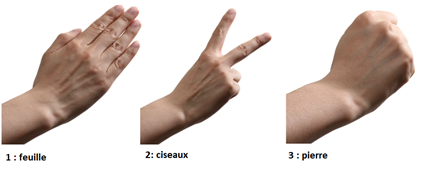
\includegraphics{images/1-image1.png}

On suppose que l'ordinateur choisit un entier \emph{ord} aléatoirement :

\begin{itemize}
\item
  Si \emph{ord}=1 alors l'ordinateur joue feuille
\item
  Si \emph{ord}=2 alors l'ordinateur joue ciseaux
\item
  Si \emph{ord}=3 alors l'ordinateur joue pierre
\end{itemize}

L'entier \emph{choix} représentera le choix de l'utilisateur. De la même
manière :

\begin{itemize}
\item
  Si \emph{choix}=1 alors l'utilisateur joue feuille
\item
  Si \emph{choix}=2 alors l'utilisateur joue ciseaux
\item
  Si \emph{choix}=3 alors l'utilisateur joue pierre
\end{itemize}

De façon générale, la pierre bat les ciseaux (en les émoussant), les
ciseaux battent la feuille (en la coupant), la feuille bat la pierre (en
l'enveloppant).

Compléter le programme suivant pour qu'il modélise le jeu contre
l'ordinateur.

\begin{Shaded}
\begin{Highlighting}[]
\ImportTok{from}\NormalTok{ random }\ImportTok{import} \OperatorTok{*}


\KeywordTok{def}\NormalTok{ jeu(choix):}
    \BuiltInTok{ord} \OperatorTok{=}\NormalTok{ randint(}\DecValTok{1}\NormalTok{, }\DecValTok{3}\NormalTok{)  }\CommentTok{\# randint(1,3) renvoie un entier aléatoire parmi 1, 2 ou 3.}
\NormalTok{    ...}


\NormalTok{jeu(}\DecValTok{1}\NormalTok{)}
\end{Highlighting}
\end{Shaded}


\end{document}
